\documentclass[conference]{IEEEtran}
\IEEEoverridecommandlockouts

\usepackage{cite}
\usepackage{amsmath,amssymb,amsfonts}
\usepackage{graphicx}
\usepackage{textcomp}
\usepackage{xcolor}
\usepackage{booktabs}
\usepackage{multirow}
\usepackage{array}
\usepackage{url}
\usepackage{hyperref}
\usepackage{microtype}
\usepackage{float}

\newcommand{\ie}{\textit{i.e.}}
\newcommand{\eg}{\textit{e.g.}}

% Reviewer-comment tags: printed only in main_annotated.pdf (main_annotated.tex defines \ANNOTATE).
\ifdefined\ANNOTATE
  \newcommand{\rc}[1]{\textcolor{blue}{\textbf{[#1]}}\,}
\else
  \newcommand{\rc}[1]{}
\fi

% Items only the authors can supply. Set \showtodosfalse once filled: the build then fails if any remain.
\newif\ifshowtodos \showtodosfalse
\ifshowtodos
  \newcommand{\todo}[1]{\textcolor{red}{\textbf{[TODO: #1]}}}
\else
  \newcommand{\todo}[1]{\errmessage{Unresolved TODO: #1}}
\fi

\begin{document}

\title{DealTwin-X: Multi-Modal Embeddings for M\&A Precedent Retrieval}

\author{\IEEEauthorblockN{Dhanisha Sethupathy\textsuperscript{1}}
\IEEEauthorblockA{\textit{School of Computer Science and Engineering}\\
\textit{Vellore Institute of Technology, Chennai, India}\\
Email: dhanisha.sethupathy2023@vitstudent.ac.in}
\and
\IEEEauthorblockN{Lakshmi Harika Palivela\textsuperscript{2,*}}
\IEEEauthorblockA{\textit{School of Computer Science and Engineering}\\
\textit{Vellore Institute of Technology, Chennai, India}\\
Email: lakshmi.harika@vit.ac.in}
\and
\IEEEauthorblockN{Adesh Kanna Prakash\textsuperscript{3}}
\IEEEauthorblockA{\textit{School of Computer Science and Engineering}\\
\textit{Vellore Institute of Technology, Chennai, India}\\
Email: adeshkannna.prakash2023@vitstudent.ac.in}
\and
\IEEEauthorblockN{Ananyaa Subramanian\textsuperscript{4}}
\IEEEauthorblockA{\textit{School of Computer Science and Engineering}\\
\textit{Vellore Institute of Technology, Chennai, India}\\
Email: ananyaa.subramanian2023@vitstudent.ac.in}
\and
\IEEEauthorblockN{Sowmiya V\textsuperscript{5}}
\IEEEauthorblockA{\textit{School of Computer Science and Engineering}\\
\textit{Vellore Institute of Technology, Chennai, India}\\
Email: sowmiya.v2023a@vitstudent.ac.in}}

\maketitle

\begin{abstract}
\rc{R1.10, R2.2}Precedent-transaction analysis values a company from the multiples paid in comparable past mergers and acquisitions (M\&A), whose comparable set is usually chosen with an industry code and a size screen. We test whether a multi-modal transaction embedding, which adds fundamentals, deal structure, acquirer type, legal-clause and business-description text, and macroeconomic context, retrieves better precedents than such screens. DealTwin-X builds a reproducible, point-in-time corpus of 2{,}416 US public-target deals (2013--2025; 1{,}947 merger proxies, 469 cash tender offers) from free SEC filings. A query retrieves only earlier deals; there is no expert ground truth, so we evaluate against five weakly correlated proxy constructs, including a new legal-aware one. All preprocessing is fitted inside folds, and all 880 comparisons use a cluster bootstrap with Holm correction. Under the outcome-grounded construct, an improved LambdaMART ranker beats the naive industry-and-size baseline (NDCG@5 $+0.095$; large effect), whereas our earlier design gains only $+0.015$, but it merely ties a four-digit-SIC-and-size screen. A two-stage cascade that re-ranks the screen's candidates using the realized multiples of earlier precedents beats that screen by a small margin (NDCG@5 $+0.012$ to $+0.015$; Holm-significant under temporal cross-validation but not under industry-grouped folds, $p=0.086$) and gives the best $k$-NN valuations ($R^2=0.40$ vs.\ $0.22$ for a causal industry median). Legal-clause text shows no outcome-relevant signal and a small legal-term signal. A gradient-boosted surrogate reaches log-space $R^2=0.38$ ($0.48$ temporally) but under-predicts high multiples. Code, a hashed data snapshot and all evaluation scripts are released.
\end{abstract}

\begin{IEEEkeywords}
Precedent transaction analysis, information retrieval, learning to rank, FinBERT, causal evaluation, SEC EDGAR, explainable AI.
\end{IEEEkeywords}

\section{Introduction}
\label{sec:intro}

In precedent-transaction analysis, one of the three standard M\&A valuation methods, the analyst selects past transactions similar to the target, reads off the multiples paid and infers a valuation range. The comparable set is usually found on proprietary terminals with an industry-classification and size filter~\cite{damodaran2012}. Transaction structure, acquirer type, legal terms and macroeconomic conditions are rarely used systematically, although each plausibly affects which earlier deals a target resembles in price~\cite{damodaran2012,hoberg2016}.

We ask a narrow, testable question: does a multi-modal transaction embedding retrieve better precedents than the industry-and-size screens an analyst already applies? Three design choices shape the answer. First, retrieval is causal-temporal: every query retrieves, and is scored against, only deals filed before it. Second, there is no expert ground truth, so \rc{R1.1}we evaluate against five weakly correlated proxy constructs and do not treat any of them as ground truth. \rc{R2.1}Third, a learned retriever is compared not only with the naive baseline of our earlier submission but also with stronger practitioner-style screens (hierarchical SIC codes, size bins and 10-K text peers).

\noindent\textbf{Contributions.}
\begin{itemize}
\item A pipeline that builds a 2{,}416-deal corpus of merger proxies and tender offers from free SEC data. It applies an M\&A gate whose exclusions are fully counted, point-in-time XBRL fundamentals (validated against an end-date-only rule), completion-status detection and an audited deal-price extractor (Section~\ref{sec:pipeline}).
\item A causal-temporal protocol with fold-local preprocessing, leakage control for multiple-based constructs, a labelled candidate pool, five proxy constructs, eight retrievers, and cluster-bootstrap inference with Holm correction over every reported comparison (Sections~\ref{sec:embedding}--\ref{sec:eval}).
\rc{R1.10, R2.2}\item An empirical account that separates statistical from practical significance (Sections~\ref{sec:results}--\ref{sec:limitations}). An improved LambdaMART ranker clearly beats the naive baseline but only ties a hierarchical-SIC screen; a two-stage cascade that also consults the precedents' realized multiples beats the screen by a small margin, significant under temporal but not industry-grouped folds, and gives the best valuations. The legal-clause block carries no outcome-relevant signal and a small legal-term signal.
\end{itemize}

\section{Related Work}
\label{sec:related}

\noindent\textbf{Comparable selection and text representation.}
Comparable-company and precedent-transaction selection traditionally screens on industry classification and size, followed by analyst judgement~\cite{damodaran2012}. \rc{R2.1}Hoberg and Phillips~\cite{hoberg2016} show that 10-K business-description similarity can identify economically similar firms better than fixed industry codes; we include a 10-K text-peer baseline and a business-description block on this basis. Sentence-BERT~\cite{reimers2019}, built on BERT~\cite{devlin2019}, produces sentence embeddings (we use MiniLM for clause selection and MPNet~\cite{song2020} as a general encoder), FinBERT~\cite{huang2023} is adapted to finance and LEGAL-BERT~\cite{chalkidis2020} to law. Generic NLP tools transfer poorly to financial text~\cite{loughran2011}.

\noindent\textbf{Retrieval, ranking and inference.}
We score graded retrieval with NDCG~\cite{jarvelin2002} and use BM25~\cite{robertson2009} as a lexical baseline. Retrieval weights are learned from pairwise preferences~\cite{liu2009} and with LambdaMART~\cite{burges2010}, implemented in LightGBM~\cite{ke2017}. The valuation surrogate uses XGBoost~\cite{chen2016} tuned with Optuna~\cite{akiba2019}. Inference uses a cluster bootstrap~\cite{cameron2008}, the Holm correction~\cite{holm1979} and Cliff's $\delta$~\cite{cliff1993}. Debreceny et al.~\cite{debreceny2010} document XBRL data-quality issues that bound our structured features. To our knowledge, no public study evaluates multi-modal M\&A precedent retrieval causally against practitioner-style screens on free filings; our contribution is the evaluation, not the architecture.

\section{Data Pipeline and Corpus}
\label{sec:pipeline}

Figure~\ref{fig:pipeline} summarizes the pipeline. Every field comes from a free public API and is cached in a hashed snapshot.

\begin{figure}[t]
\centering
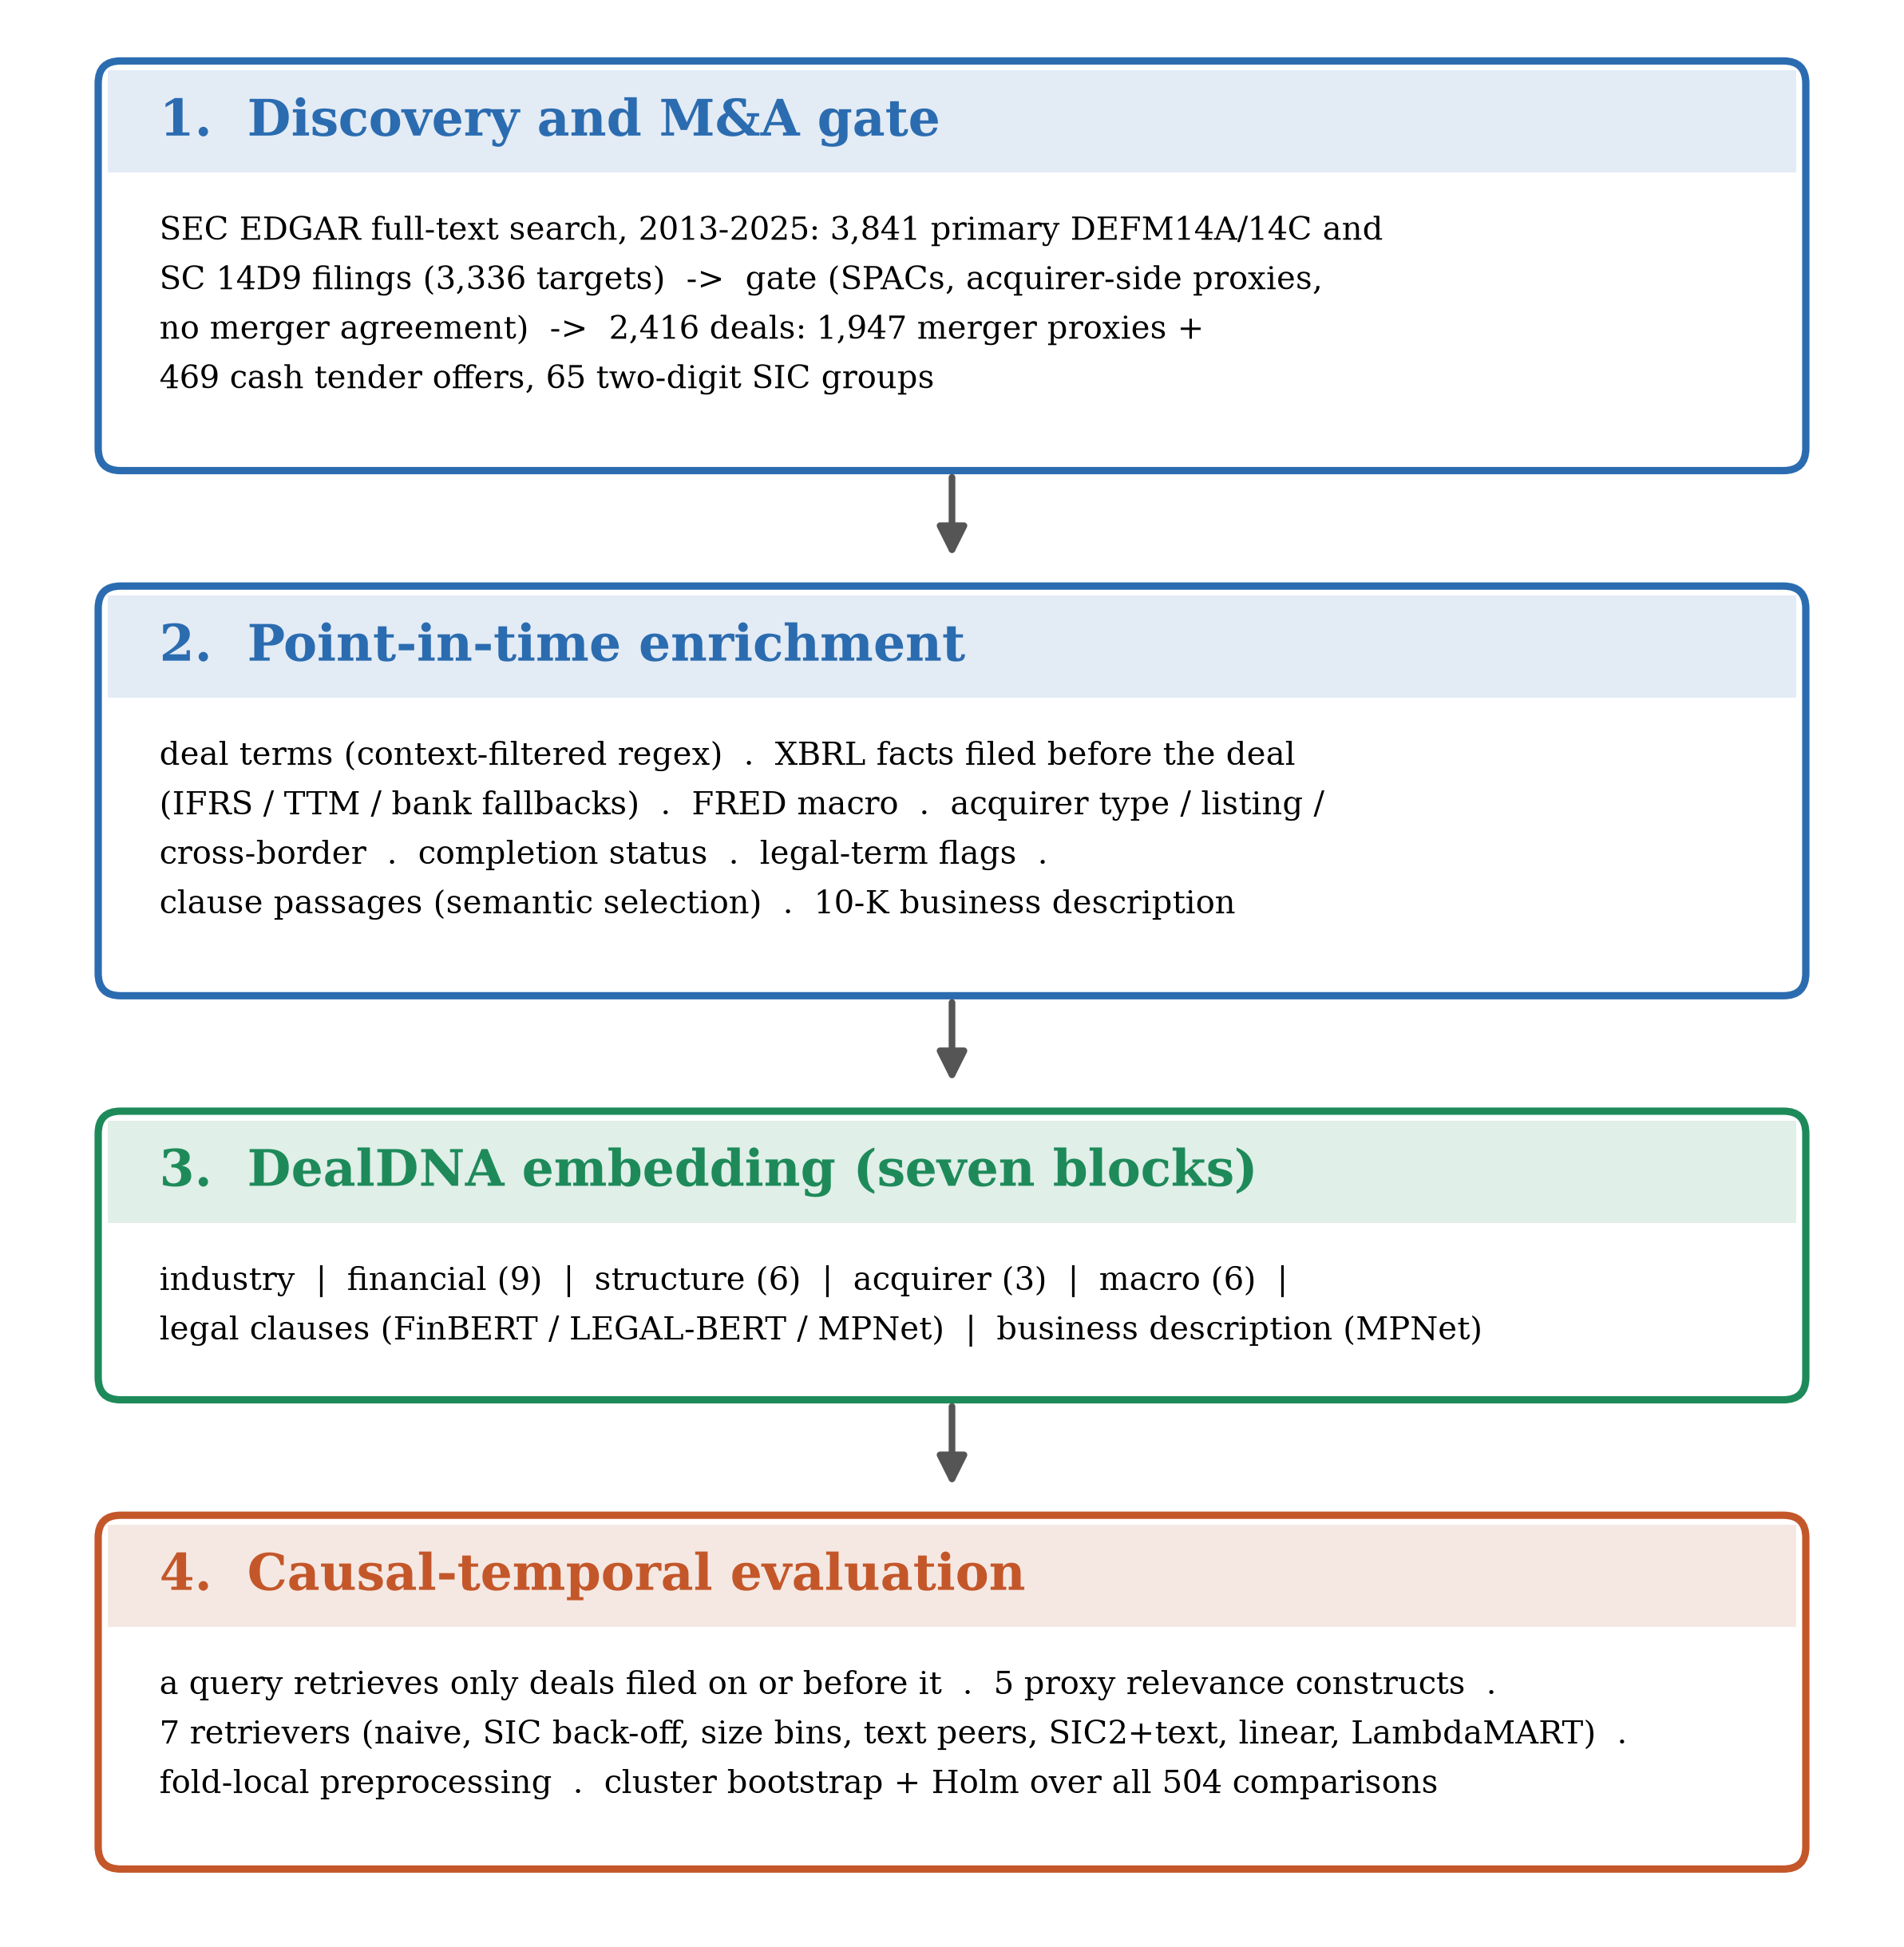
\includegraphics[width=\columnwidth]{figures/fig0_pipeline.png}
\caption{The DealTwin-X pipeline: discovery and M\&A gate, point-in-time enrichment, the DealDNA embedding, and the causal-temporal evaluation.}
\label{fig:pipeline}
\end{figure}

\rc{R2.8}\noindent\textbf{Discovery and parsing yield.}
SEC EDGAR full-text search over 2013-01-01 to 2025-06-30, split by year, with 15 phrasings for merger proxies (DEFM14A/DEFM14C) and 5 for cash-tender-offer recommendation statements (SC~14D9), returns 3{,}841 original primary documents (amendments and exhibits removed) for 3{,}336 target companies. For each target we keep the earliest filing that passes an M\&A gate. The gate requires a merger agreement and excludes SPAC business combinations, acquirer-side proxies (a share-issuance proposal without the Item~402(t) merger-compensation vote that target proxies must hold) and asset sales. In total, 2{,}416 targets (72.4\%) yield a deal. The 1{,}095 filings of the 920 excluded targets fail because they contain no merger agreement (652, mostly mini-tender and partial offers), are SPAC filings (320) or acquirer-side proxies (104), are too short (11), lack point-in-time XBRL data (5) or are asset sales (3).

\rc{R2.8}\noindent\textbf{Point-in-time fundamentals.}
Fundamentals come from the SEC XBRL Company Facts API, with IFRS, trailing-twelve-month and bank-revenue (interest plus noninterest income) fallbacks. A fact is used only if it was \emph{filed} on or before the deal's filing date; when a period was reported more than once, the earliest-filed value is used, so later restatements are ignored. This matters. Selecting by period end date alone, as is common, would have used a revenue fact filed \emph{after} the deal for 451 of the 1{,}760 deals with annual revenue (25.6\%), and a different revenue value for 246 of them (14.0\%; median gap 12.7\%). Macroeconomic context at the filing date comes from FRED: federal funds rate, 10-year Treasury yield, yield-curve slope, VIX and, because FRED now restricts the ICE high-yield series to the most recent three years, the Moody's Baa minus 10-year Treasury credit spread.

\rc{R2.8}\noindent\textbf{Deal terms and their accuracy.}
The deal price is the per-share cash figure that the document repeats most often within a consideration context (``in cash'', ``net to the seller'', ``merger consideration'', \dots), excluding figures attached to par values, dividends, preferred-stock terms, exercise or trading prices, and those in sentences describing earlier proposals. We designed these rules on one random sample of 50 filings and then audited a separate random sample of 60. In that audit sample, 50 extracted prices (83\%) were exactly correct; among the 51 all-cash deals, for which we compute enterprise value, 47 were (92\%). Enterprise value is computed only for all-cash deals, as price $\times$ shares outstanding $+$ long-term debt $-$ cash; for stock deals, the acquirer's historical share price is not available from free sources. Acquirer type (financial sponsor or strategic), listing and cross-border status are extracted from the disclosure text, together with ten binary legal-term flags (go-shop, reverse termination fee, HSR, CFIUS, majority-of-minority, support agreements, financing condition, top-up option, Section~251(h), CVR).

\rc{R2.8}\noindent\textbf{Terminated deals.}
A proxy or SC~14D9 precedes closing, so some deals were later terminated. A deal counts as completed if the target filed a Form~25 or Form~15 deregistration within 18 months, and as terminated if it instead kept filing 10-K/10-Q reports more than 12 months later. Of the 2{,}416 deals, 2{,}244 completed, 165 (6.8\%) were terminated and 7 are undetermined. Terminated deals are retained, because the terms they disclose remain informative, and are analysed separately in Section~\ref{sec:robustness}.

\begin{table}[t]
\centering
\caption{Corpus composition and field coverage (2{,}416 deals, 65 two-digit SIC groups, 2013--2025).}
\label{tab:corpus}
\footnotesize
\setlength{\tabcolsep}{3pt}
\resizebox{\columnwidth}{!}{%
\begin{tabular}{@{}lr@{\hspace{1em}}lr@{}}
\toprule
Component & Value & Field & Cov. \\
\midrule
Merger proxies (DEFM14A/14C)   & 1{,}947      & Revenue (point-in-time XBRL) & 90.9\% \\
Cash tender offers (SC 14D9)   & 469          & EBITDA proxy                 & 78.8\% \\
Computable EV/Revenue (all-cash) & 1{,}091    & Revenue growth (YoY)         & 81.2\% \\
Strategic / sponsor acquirer   & 1{,}764/652  & Cash price per share         & 73.1\% \\
Cross-border acquirer          & 381          & Termination fee              & 87.7\% \\
Completed / terminated         & 2{,}244/165  & Filing-stated premium        & 35.1\% \\
10-K business description      & 91.7\%       & Clause passage ($\ge$1)      & 100\% \\
\bottomrule
\end{tabular}}
\end{table}

\rc{R1.6}Table~\ref{tab:corpus} summarizes the corpus. A clean filing-stated premium is available for 35.1\% of the deals; we use it as a feature only where the evaluation target does not depend on the multiple (Section~\ref{sec:embedding}).

\section{The DealDNA Embedding and Baselines}
\label{sec:embedding}

\noindent\textbf{Blocks.}
Each deal is represented by seven blocks. The \emph{industry} block contains the two-digit SIC group and, for the ranker, two-, three- and four-digit SIC match indicators. The \emph{financial} block (9 features) contains log revenue, revenue growth, EBITDA margin, net margin, leverage, cash ratio, EV/Revenue, EV/EBITDA and deal premium. The \emph{structure} block (6) contains cash/stock/mixed indicators, an earn-out flag, the termination fee as a fraction of EV and the intensity of MAC-clause mentions. The \emph{acquirer} block (3) contains sponsor, listed and cross-border flags. The \emph{macro} block (6) contains the five FRED series and a filing-date ordinal. The \emph{legal} block is the mean-pooled embedding of the selected clause passages (FinBERT-tone~\cite{huang2023} by default, with LEGAL-BERT~\cite{chalkidis2020} and MPNet~\cite{song2020} as alternatives). \rc{R1.4}The \emph{business} block is the MPNet embedding of the target's latest 10-K Item~1 filed before the deal. \rc{R2.4}Numeric blocks are median-imputed and $z$-scored with statistics estimated on the training fold only.

\rc{R1.4, R1.5}\noindent\textbf{Clause selection.}
Clause passages are selected by sentence-embedding similarity to eight clause-type prototypes (two passages per type above a similarity threshold). Table~\ref{tab:clauses} reports the precision of this selection against a keyword-anchored silver standard on 120 random filings. Precision is high for appraisal rights and termination fees but low for regulatory approval (0.24) and especially earn-outs (0.04): most deals have no earn-out, yet the selector still returns the two most similar sentences. We therefore apply a lexical gate (the clause's keyword must be present) to the three lowest-precision types. Their gated precision is 1.0 by construction, which raises overall precision from 0.59 to 0.84, but the silver standard itself is keyword-based and the passages of the five ungated types remain noisy.

\begin{table}[t]
\centering
\caption{Clause-selector passage precision by clause type against a keyword-anchored silver standard (120 random filings, 240 passages per type before gating). Gated types require their keyword after gating, so their precision is 1.0 by construction.}
\label{tab:clauses}
\footnotesize
\setlength{\tabcolsep}{4pt}
\resizebox{\columnwidth}{!}{%
\begin{tabular}{lcc}
\toprule
Clause type & Ungated & Gated (passages kept) \\
\midrule
Appraisal rights               & 0.97 & 0.97 (240) \\
Termination fee                & 0.85 & 0.86 (240) \\
Representations and warranties & 0.74 & 0.74 (240) \\
Exchange ratio / consideration & 0.69 & 0.69 (240) \\
No-solicitation / fiduciary out & 0.60 & 0.59 (240) \\
Material adverse effect$^\dagger$ & 0.56 & 1.00 (218) \\
Regulatory approval$^\dagger$  & 0.24 & 1.00 (221) \\
Earn-out / CVR$^\dagger$       & 0.04 & 1.00 (54) \\
\midrule
Overall                        & 0.59 & 0.84 \\
\bottomrule
\multicolumn{3}{l}{$^\dagger$ lexical gate applied}
\end{tabular}}
\end{table}

\rc{R2.3}\noindent\textbf{Leakage control.}
The concordance and outcome-grounded constructs (Section~\ref{sec:eval}) are defined by the realized EV/Revenue multiple. When either is the target, every feature computed from the transaction value is removed: EV/Revenue, EV/EBITDA, deal premium and the termination fee, which is negotiated as a fraction of equity value and would therefore encode the price. Margins and growth are pre-deal fundamentals and are retained. The candidate pool is also restricted to deals with a computable multiple; otherwise a retriever could score well by predicting which candidates have a label (\eg, ``cash deals have multiples''), an effect we observed. The cascade ranker (Section~\ref{sec:eval}) uses the realized multiples of \emph{earlier} candidate deals, which are public at the query date, but never the query's own; a unit test verifies that changing a query's multiple leaves its ranking unchanged.

\rc{R2.1}\noindent\textbf{Baselines.}
(i)~\emph{Naive}, the baseline of our earlier submission: the inner product of a weighted two-digit-SIC one-hot vector and standardized log revenue. (ii)~\emph{SIC back-off}: same two-digit, then three-digit, then four-digit SIC code, then closest revenue. (iii)~\emph{Size bins}: same two-digit SIC code, then same within-industry revenue quintile (cut points from the training fold), then closest revenue. (iv)~\emph{Text peers}: cosine similarity of the 10-K business-description embeddings, in the spirit of Hoberg and Phillips~\cite{hoberg2016}. (v)~\emph{SIC2 + text}: same two-digit SIC code, then text similarity. SEC data provide SIC but not NAICS codes, so the finer-industry baselines use SIC. In addition, four clause-passage text baselines (TF-IDF, BM25~\cite{robertson2009}, MiniLM~\cite{reimers2019} and FinBERT, each with industry first) test the legal text on its own.

\section{Evaluation Protocol}
\label{sec:eval}

\rc{R2.4}\noindent\textbf{Causal-temporal protocol.}
Query $i$ may retrieve deal $j\neq i$ only if $t_j\le t_i$ (filing dates). Cross-validation uses five folds, either GroupKFold by two-digit SIC (the main setting) or an expanding time window in which the earliest block is used only for training. Imputation, scaling, size bins, block weights and the ranker are all fitted on the training fold. Learned retrievers are trained only on (query, candidate) pairs whose query and candidate both lie in the training fold, so no test-fold outcome is ever used in training. Test queries are ranked against all admissible candidates.

\noindent\textbf{Relevance constructs.}
All constructs are gated on the two-digit SIC group and graded. (1)~\emph{Heuristic}: industry, size, consideration structure and recency. (2)~\emph{Practitioner rubric}~\cite{damodaran2012}: industry, size tier, business-profile distance on growth and margin, and structure and recency as tie-breakers. (3)~\emph{Concordance}: binary; industry, size, realized multiple and structure must all agree (5{,}666 positive pairs). (4)~\emph{Outcome-grounded}: graded by the similarity of realized EV/Revenue multiples (89{,}280 positive pairs). \rc{R2.6}(5)~\emph{Legal-aware} (new): graded by agreement on the ten legal-term flags, which are extracted independently of the clause selector. The two screening-style constructs (1) and (2) share a design and correlate at Kendall $\tau=0.62$; all other pairs correlate at $\tau=-0.11$ to $0.33$, and the legal-aware construct is nearly independent of the rest ($|\tau|\le0.15$). \rc{R1.1}These constructs are proxies, not ground truth. Constructs (1)--(3) partly reuse attributes that the retrievers also see, so they favour some retrievers by design; we therefore treat the outcome-grounded construct as primary and the legal-aware construct as the test of legal content. No practitioner judgements were available for this study; we release a labelling template for them.

\noindent\textbf{Metrics.}
We report NDCG@5 and within-industry (WI) NDCG@5/@10 over graded relevance, plus MAP, MRR, P@5 and R@10 over binary relevance ($r>0$). \rc{R1.10, R2.2}Because every construct is industry-gated, binary relevance coincides with ``same industry'', so every retriever that ranks same-industry deals first attains identical binary metrics (MAP $=$ MRR $=1$). These metrics therefore measure only industry gating, and our conclusions rest on the graded metrics. WI-NDCG ranks only same-industry candidates and is reported for queries with at least three such candidates spanning at least two relevance levels.

\rc{R2.4}\noindent\textbf{Statistical inference.}
Deals in the same industry and year share market conditions and candidate lists, so the per-deal differences are not independent. Confidence intervals come from a cluster bootstrap~\cite{cameron2008} that resamples (two-digit SIC $\times$ filing year) blocks of queries 10{,}000 times, and $p$-values from a $z$-test with the bootstrap standard error. Holm's correction~\cite{holm1979} is applied jointly to all 880 comparisons reported in the paper and its released results (every retriever pair, metric and construct, the ablations and the dispersion split). Effect size is the paired Cliff's $\delta=P(d>0)-P(d<0)$, with $|\delta|<0.147$ negligible, $<0.33$ small, $<0.474$ medium and large otherwise~\cite{cliff1993}. The per-deal Wilcoxon test is reported only as a secondary check.

\noindent\textbf{Learned retrievers.}
The \emph{linear} retriever fits non-negative per-block weights by pairwise-ranking logistic regression (average of three seeds, weights summing to the number of blocks). The \emph{LambdaMART} ranker (LightGBM \texttt{lambdarank}; 31 leaves, learning rate 0.03; full settings in the repository) uses 19 pair features: SIC2/3/4 match indicators; the cosine similarity of the financial, structure, acquirer, macro, legal and business blocks; absolute differences of six financial features; agreement of consideration mix, deal type and acquirer type; and the time gap. Each training query contributes up to 150 relevant and 150 non-relevant candidates, with early stopping on 15\% of the training queries. The ranker of our earlier submission, re-run here as \emph{LambdaMART (submitted)}, used only one similarity per block and a two-digit SIC match. \rc{R2.1}The \emph{cascade} is a two-stage design fixed before evaluation. The SIC back-off screen proposes its top 50 candidates, and a LambdaMART ranker with the same settings re-ranks them using the 19 pair features plus the screen rank, the candidate's realized multiple, the query's predicted multiple (an in-fold LightGBM surrogate on pre-deal features, with inner out-of-fold predictions for training queries) and the median multiple of the screened candidates. \rc{R2.5}We also explored a contrastive neural encoder during development; because it cannot be documented to a reproducible level within the page limit, we make no claims about it.

\section{Results}
\label{sec:results}

\subsection{Valuation-Multiple Surrogate}
\label{sec:surrogate}

On the 1{,}091 deals with a computable multiple, an XGBoost surrogate predicts $\log(1+\text{EV/Revenue})$ from the pre-deal features only. These are the financial, structure, acquirer and macro features with all value-derived features removed, plus a fold-local industry target encoding and ten principal components of the business-description embedding. Hyperparameters are re-tuned with Optuna (30 trials) inside every outer training fold. Under GroupKFold by SIC, XGBoost reaches a log-space $R^2$ of $0.38$ (MAE $3.46\times$); gradient boosting reaches $0.34$, Ridge $0.10$ and the industry median $-0.05$. \rc{R2.7}Under expanding-window temporal cross-validation, XGBoost reaches $R^2=0.48$ against $0.23$ for the industry median.


\rc{R2.7}The industry median's gap ($-0.05$ vs.\ $0.23$; $0.22$ in Section~\ref{sec:valuation}) comes from the split, not the predictor. Under GroupKFold by SIC, the test industry never appears in the training fold, so the ``industry median'' falls back to the global training median for 100\% of test deals. Under temporal folds, same-industry history exists for 97.4\% of test deals. GroupKFold therefore measures generalization to unseen industries, which is harder than the practitioner's task; temporal cross-validation is the realistic setting.

\rc{R1.7}\noindent\textbf{Error by valuation range.}
The surrogate shrinks toward the conditional mean (Table~\ref{tab:surrogate_err}). It over-predicts the lowest quintile and severely under-predicts the highest: in the top predicted quintile, it predicts $5.5\times$ on average against a realized $13.6\times$. A $\pm1\sigma$ residual band covers 74\% of deals overall (nominal 68\%) but only 25\% in the top realized quintile. The surrogate is therefore an explanation aid that shows which fundamentals move a multiple. It is not a valuation tool and is unreliable above roughly $6\times$ revenue, the boundary of the top quintile. By gain importance, it is led by the industry encoding, EBITDA margin, net margin, revenue growth and size.

\begin{table}[t]
\centering
\caption{Surrogate error by realized EV/Revenue quintile (out-of-fold, GroupKFold by SIC). Bias $=$ mean(predicted $-$ realized).}
\label{tab:surrogate_err}
\footnotesize
\setlength{\tabcolsep}{4pt}
\begin{tabular}{lcccc}
\toprule
Quintile & Range ($\times$) & MAE ($\times$) & Bias ($\times$) & $\pm1\sigma$ cov. \\
\midrule
Q1 & 0.05--0.77 & 1.13 & $+1.13$ & 0.69 \\
Q2 & 0.77--1.56 & 1.00 & $+0.94$ & 0.89 \\
Q3 & 1.56--2.78 & 0.79 & $+0.30$ & 0.97 \\
Q4 & 2.78--5.72 & 1.34 & $-0.83$ & 0.92 \\
Q5 & 5.72--94.8 & 12.97 & $-12.89$ & 0.25 \\
\bottomrule
\end{tabular}
\end{table}

\subsection{Retrieval: The Outcome-Grounded Test}

\rc{R2.1, R2.2}Table~\ref{tab:outcome} reports retrieval under the outcome-grounded construct (1{,}032 queries). The naive baseline is the weakest industry-aware retriever. The finer SIC back-off screen is much stronger, raising NDCG@5 from $0.683$ to $0.777$, the improved LambdaMART ranker reaches the same level ($0.778$), and the cascade exceeds it ($0.789$). Size bins, text peers and the linear retriever lie in between, and the ranker of our earlier submission ($0.698$) barely improves on naive. The binary metrics are saturated, as explained in Section~\ref{sec:eval}. The ordering is unchanged under temporal folds.

\begin{table}[t]
\centering
\caption{Outcome-grounded retrieval (causal; candidates restricted to deals with a multiple; 1{,}032 queries, 901 WI-evaluable). Left: GroupKFold by SIC; right: expanding time window.}
\label{tab:outcome}
\footnotesize
\setlength{\tabcolsep}{3pt}
\resizebox{\columnwidth}{!}{%
\begin{tabular}{lcccc@{\hspace{1.2em}}cc}
\toprule
& \multicolumn{4}{c}{SIC folds} & \multicolumn{2}{c}{Time folds} \\
\cmidrule(lr){2-5}\cmidrule(lr){6-7}
Retriever & NDCG@5 & WI-N@5 & WI-N@10 & MAP & NDCG@5 & WI-N@5 \\
\midrule
Naive (SIC2 + size)       & 0.683 & 0.649 & 0.705 & 0.983 & 0.653 & 0.634 \\
SIC back-off (2/3/4 + size) & 0.777 & 0.746 & 0.787 & 1.000 & 0.756 & 0.735 \\
Size bins                 & 0.698 & 0.655 & 0.710 & 1.000 & 0.668 & 0.641 \\
10-K text peers           & 0.362 & 0.682 & 0.732 & 0.401 & 0.346 & 0.667 \\
SIC2 + text               & 0.722 & 0.682 & 0.732 & 1.000 & 0.693 & 0.667 \\
\midrule
DealDNA, linear           & 0.724 & 0.686 & 0.734 & 1.000 & 0.699 & 0.674 \\
LambdaMART (submitted)    & 0.698 & 0.656 & 0.711 & 1.000 & -- & -- \\
LambdaMART (improved)     & 0.778 & 0.747 & 0.786 & 1.000 & 0.750 & 0.729 \\
LambdaMART cascade        & \textbf{0.789} & \textbf{0.759} & \textbf{0.799} & 1.000 & \textbf{0.771} & \textbf{0.752} \\
\bottomrule
\end{tabular}}
\end{table}

\subsection{Statistical and Practical Significance}
\label{sec:significance}

\rc{R1.2, R2.2}Table~\ref{tab:sig} gives the paired tests. Four results stand out. First, the improved ranker beats the naive baseline with a large effect on every graded metric (NDCG@5 $+0.095$, WI-NDCG@5 $+0.098$, Holm $p<10^{-60}$, $\delta=0.51$--$0.56$). Second, the ranker design of our earlier submission does not: its NDCG@5 gain is $+0.015$ (negligible) and its WI-NDCG gain is not significant, which reproduces the reviewers' concern. The design changes (fine SIC match indicators, feature-difference features) account for a $+0.080$/$+0.091$ improvement. Third, against the hierarchical SIC back-off screen, the improved ranker's difference is $+0.0005$ NDCG@5 (95\% CI $[-0.006, 0.007]$, Holm $p=1$). A block ablation confirms this: removing the industry features costs $0.48$ NDCG@5, whereas removing any other block changes it by less than $0.01$, with no change significant after correction. Fourth, the cascade beats the screen: $+0.012$ NDCG@5 under SIC folds (95\% CI $[0.006, 0.018]$; Holm $p=0.086$) and $+0.015$ under temporal folds (Holm $p=0.003$), with WI-NDCG@10 $+0.012$ (Holm $p<10^{-3}$). The effect is negligible in size ($\delta\le0.14$); it has the same sign under both fold schemes but is significant after correction only under temporal folds and on WI-NDCG@10, so we treat it as suggestive rather than established. Its ablation locates the source: without the precedent-multiple features the cascade exactly ties the screen ($-0.0001$), so the gain comes from consulting what earlier comparable deals were actually paid, not from re-ranking itself.

\begin{table}[t]
\centering
\caption{Paired differences under the outcome-grounded construct (cluster-bootstrap Holm $p$ over the 880-comparison family; $\delta$: paired Cliff's delta).}
\label{tab:sig}
\footnotesize
\setlength{\tabcolsep}{3pt}
\resizebox{\columnwidth}{!}{%
\begin{tabular}{lccc@{\hspace{0.8em}}ccc}
\toprule
& \multicolumn{3}{c}{NDCG@5} & \multicolumn{3}{c}{WI-NDCG@5} \\
\cmidrule(lr){2-4}\cmidrule(lr){5-7}
Comparison & diff & Holm $p$ & $\delta$ & diff & Holm $p$ & $\delta$ \\
\midrule
Linear vs.\ naive                  & $+0.042$ & $<10^{-15}$ & $0.21$ & $+0.037$ & $<10^{-10}$ & $0.20$ \\
LMART (submitted) vs.\ naive       & $+0.015$ & $0.10$      & $0.08$ & $+0.007$ & $1.00$      & $0.05$ \\
LMART (improved) vs.\ naive        & $+0.095$ & $<10^{-68}$ & $0.51$ & $+0.098$ & $<10^{-70}$ & $0.56$ \\
LMART improved vs.\ submitted      & $+0.080$ & $<10^{-46}$ & $0.46$ & $+0.091$ & $<10^{-56}$ & $0.52$ \\
LMART (improved) vs.\ SIC back-off & $+0.001$ & $1.00$      & $-0.01$ & $+0.001$ & $1.00$     & $-0.01$ \\
\midrule
Cascade vs.\ SIC back-off          & $+0.012$ & $0.086$     & $0.07$ & $+0.013$ & $0.095$    & $0.08$ \\
\quad same, time folds              & $+0.015$ & $0.003$     & $0.10$ & $+0.017$ & $0.003$    & $0.11$ \\
Cascade w/o multiples vs.\ back-off & $0.000$ & $1.00$     & $0.01$ & $+0.000$ & $1.00$     & $0.01$ \\
\bottomrule
\end{tabular}}
\end{table}


\rc{R1.2, R1.10}\noindent\textbf{Practical significance.}
The binary metrics barely move: top-10 lists contain 8.29 versus 8.22 relevant precedents, because both retrievers already fill them with same-industry deals. The improvement lies in the ordering \emph{within} the industry. WI-NDCG@5 rises by 15\% (0.649 to 0.747), so the deals whose multiples are closest to the query move to the top of the list. The gain is significant both in industries whose realized multiples are dispersed (NDCG@5 $+0.102$, $\delta=0.55$) and in tightly clustered ones ($+0.085$, $\delta=0.44$). For an analyst, the practical message is that a two-digit SIC-and-size screen is a weak default; a four-digit SIC back-off with a size tie-break captures most of the gain at no cost, and ordering its candidates by their realized multiples adds a small further improvement.

\subsection{Consistency Across Relevance Constructs}

\rc{R1.1, R2.6}Table~\ref{tab:constructs} reports NDCG@5 under all five constructs. Improved LambdaMART beats naive under every construct (Holm $p<10^{-39}$). Under the heuristic and rubric constructs, which are deterministic functions of attributes the ranker sees, it also beats the strongest baseline by $0.09$ and $0.06$; we read this as the ranker reproducing the construct rather than as evidence of comparability. Under concordance it ties the size-bin screen ($-0.0004$, $p=1$), whereas the cascade beats it ($+0.060$, Holm $p<10^{-3}$). Under the independent legal-aware construct, it beats SIC back-off by $+0.040$ (Holm $p<10^{-20}$, $\delta=0.24$, small).

\begin{table}[t]
\centering
\caption{NDCG@5 under the five proxy constructs (GroupKFold by SIC). Strongest baseline: SIC back-off, except size bins under concordance.}
\label{tab:constructs}
\footnotesize
\setlength{\tabcolsep}{3pt}
\resizebox{\columnwidth}{!}{%
\begin{tabular}{lccccc}
\toprule
Retriever & Heuristic & Rubric & Concord. & Outcome & Legal-aware \\
\midrule
Naive              & 0.624 & 0.639 & 0.207 & 0.683 & 0.634 \\
SIC back-off       & 0.893 & 0.908 & 0.343 & 0.777 & 0.790 \\
Size bins          & 0.869 & 0.891 & 0.396 & 0.698 & 0.707 \\
DealDNA, linear    & 0.831 & 0.810 & 0.303 & 0.724 & 0.757 \\
LMART (submitted)  & 0.839 & 0.817 & 0.270 & 0.698 & 0.763 \\
LMART (improved)   & 0.986 & 0.966 & 0.396 & 0.778 & 0.830 \\
LMART cascade      & 0.989 & 0.970 & 0.456 & 0.789 & 0.826 \\
\bottomrule
\end{tabular}}
\end{table}

\subsection{The Legal-Clause Block}

\rc{R1.4, R2.6}We restate our earlier conclusion more carefully: \emph{with these constructs and this clause selector}, the legal-clause block carries no signal for outcome-based comparability and a small signal for legal-term comparability. Under the outcome-grounded construct, the cross-validated linear weight of the legal block is $0.031$ of a budget of $6$, compared with about $5.6$ for the industry block. Table~\ref{tab:legal} shows that this holds for all three encoders. Removing the block from LambdaMART changes NDCG@5 by $0.002$ (not significant). Clause-passage text baselines (TF-IDF $0.706$, BM25 $0.702$, MiniLM $0.692$, FinBERT $0.702$ NDCG@5, each with industry first) lie well below the SIC back-off screen ($0.777$). Under the legal-aware construct, however, the block receives a larger weight, especially with MPNet ($0.21$), and removing it from LambdaMART costs $0.008$ NDCG@5 (Holm $p<10^{-5}$, $\delta=0.10$, negligible).

\begin{table}[t]
\centering
\caption{Cross-validated linear weight of the legal-clause block (budget 6; range over folds) by encoder and construct.}
\label{tab:legal}
\footnotesize
\setlength{\tabcolsep}{3pt}
\resizebox{\columnwidth}{!}{%
\begin{tabular}{lccc}
\toprule
Encoder & Heuristic & Outcome-grounded & Legal-aware \\
\midrule
FinBERT-tone & 0.039 [0.012, 0.059] & 0.031 [0.016, 0.041] & 0.098 [0.053, 0.122] \\
LEGAL-BERT   & 0.008 [0.000, 0.017] & 0.013 [0.010, 0.018] & 0.048 [0.030, 0.058] \\
MPNet        & 0.166 [0.066, 0.211] & 0.023 [0.000, 0.046] & 0.207 [0.158, 0.263] \\
\bottomrule
\end{tabular}}
\end{table}

\rc{R1.5}Three factors bound this conclusion. First, four of the five constructs contain no legal content, and the legal-aware construct is itself built from regex flags. Second, the selector is imperfect (Table~\ref{tab:clauses}), and all encoders consume the same passages. Third, clause passages are dominated by boilerplate. The 10-K business-description block likewise adds nothing measurable once four-digit SIC codes are available (ablation $0.001$), although text peers alone order deals within an industry better than naive does (WI-NDCG@5 $0.682$ vs.\ $0.649$).

\subsection{Does Better Retrieval Give Better Valuations?}
\label{sec:valuation}

\rc{R1.3}Under the causal protocol, we predict a query's $\log(1+\text{EV/Revenue})$ from its top-8 retrieved precedents with a rank-weighted mean. This setting was fixed in advance, so no $k$ or aggregator is chosen on the evaluation data. Table~\ref{tab:knn} compares the result with a causal industry median (the median of earlier same-industry deals). With industry-aware retrievers, $k$-NN valuation now beats the industry median. The best is the cascade: $R^2=0.402$ versus $0.219$, and absolute log error $-0.084$ (Holm $p<10^{-11}$, $\delta=0.21$, small), ahead of the linear DealDNA retriever ($0.357$). The plain LambdaMART ranker is weaker ($R^2=0.329$), because an NDCG objective without precedent multiples rewards industry ordering rather than homogeneity of the neighbours' multiples. A retriever trained directly to minimize the neighbour--query multiple distance (``valuation objective'') did not help ($R^2=0.257$). Across a 15-configuration grid ($k\in\{3,5,8,10,20\}$; mean, median or rank-weighted), the cascade is best in every configuration (best $R^2=0.411$ at $k=20$).

\begin{table}[t]
\centering
\caption{$k$-NN valuation (top-8, rank-weighted, causal; 1{,}088 queries) vs.\ the causal industry median. $\Delta$err: reduction in mean absolute log error vs.\ the industry median (positive favours the retriever).}
\label{tab:knn}
\footnotesize
\setlength{\tabcolsep}{3pt}
\resizebox{\columnwidth}{!}{%
\begin{tabular}{lccccc}
\toprule
Predictor & $R^2_{\log}$ & MAE ($\times$) & $\Delta$err & Holm $p$ & $\delta$ \\
\midrule
Industry median (causal) & 0.219 & 3.76 & -- & -- & -- \\
Naive retrieval          & 0.090 & 4.20 & $-0.037$ & 0.052 & $-0.05$ \\
SIC back-off             & 0.315 & 3.60 & $+0.035$ & 0.026 & $0.10$ \\
SIC2 + text              & 0.340 & 3.42 & $+0.050$ & $<0.001$ & $0.13$ \\
DealDNA, linear          & 0.357 & 3.41 & $+0.060$ & $<0.001$ & $0.14$ \\
LambdaMART (improved)    & 0.329 & 3.55 & $+0.055$ & $<0.001$ & $0.17$ \\
Valuation objective      & 0.257 & 3.57 & $+0.056$ & $<0.001$ & $0.13$ \\
LambdaMART cascade       & \textbf{0.402} & \textbf{3.37} & $\mathbf{+0.084}$ & $<0.001$ & $0.21$ \\
\bottomrule
\end{tabular}}
\end{table}

\subsection{Robustness}
\label{sec:robustness}

\noindent\textbf{Protocol.} Evaluating without the causal mask lowers NDCG@5 by $0.062$--$0.075$ for every retriever (\eg, outcome LambdaMART $0.778\to0.703$).
\rc{R2.2}\noindent\textbf{Split.} Replacing SIC-grouped folds with temporal folds changes WI-NDCG@5 by at most $0.018$ (Table~\ref{tab:outcome}).
\rc{R1.10}\noindent\textbf{Threshold.} Sweeping the outcome construct's tight-multiple window from $0.15$ to $0.30$ log units leaves the legal-block weight between $0.030$ and $0.032$. This resolves an inconsistency in our earlier submission, which reported 0.11 in the main text but 0.025--0.045 in the sweep.
\rc{R1.6}\noindent\textbf{Missing data.} Under the heuristic and rubric constructs, median imputation, median imputation plus missingness indicators, and dropping the premium and EV-derived features change WI-NDCG@5 by at most $0.012$. For the surrogate, adding missingness indicators gives $R^2=0.377$ (vs.\ $0.375$), and XGBoost's native missing-value handling gives $0.335$. Deal premium (64.9\% missing) is used only where the target does not depend on the multiple, and EV only for all-cash deals.
\rc{R1.8}\noindent\textbf{Subgroups.} The improvement of LambdaMART over naive in NDCG@5 is similar for merger proxies ($+0.094$) and tender offers ($+0.100$), strategic ($+0.098$) and sponsor ($+0.092$) acquirers, and completed ($+0.095$) and terminated ($+0.104$, $n=38$) deals.
\rc{R1.9}\noindent\textbf{Reproducibility.} The pipeline includes 42 unit tests covering, among other things, the point-in-time rule, the causal mask, leakage control and fold-local preprocessing. The processed snapshot, embeddings and every result file are frozen with a SHA-256 manifest.

\section{Limitations and Threats to Validity}
\label{sec:limitations}

\rc{R1.1}\noindent\textbf{No expert ground truth.} All five constructs are proxies for an analyst's comparability judgement, and three reuse attributes that the retrievers see. Triangulation across weakly correlated constructs reduces, but does not remove, this risk. Our conclusions concern retrieval quality with respect to these proxies, and practitioner labels are the most important missing validation.

\rc{R1.5, R2.8}\noindent\textbf{Extraction quality.} Deal-price extraction is 92\% accurate on all-cash deals and 83\% overall in a 60-filing audit. The selector's ungated precision is 0.59, and the silver standard is keyword-based. The legal conclusions are bounded accordingly.

\rc{R1.8}\noindent\textbf{External validity.} The corpus contains only US public targets that file a DEFM14A/14C or SC~14D9. It excludes S-4 stock-for-stock mergers, private targets (the majority of M\&A by count), non-US deals, asset sales and carve-outs. Multiples are computed only for all-cash deals (1{,}091), so the outcome-based results describe cash acquisitions of public companies. Private targets lack XBRL data, so the findings should not be extrapolated to them.

\section{Conclusion}
\label{sec:conclusion}

\rc{R2.2}DealTwin-X evaluates precedent retrieval on a reproducible, point-in-time corpus of 2{,}416 US M\&A deals under a causal-temporal protocol. Stronger baselines, leakage control, fold-local preprocessing and clustered inference sharpen the conclusions of our earlier submission. A redesigned LambdaMART ranker improves substantially on the naive industry-and-size baseline, whereas the earlier ranker design does not. Yet it only matches a four-digit-SIC back-off screen, because industry granularity plus size carries most of the measurable signal. A cascade that re-ranks the screen's candidates using the precedents' realized multiples beats the screen by a small margin, significant after correction under temporal folds but not industry-grouped folds, and yields the best $k$-NN valuations. Legal-clause text adds nothing for outcome-based comparability and a small, detectable amount for legal-term comparability. For practitioners, a fine-grained SIC screen with a size tie-break is a strong, free default, and re-ordering it by precedent multiples is a cheap improvement. For research, the priorities are practitioner relevance labels, stock-deal valuations and private-target data.

\section*{Data and Code Availability}
\label{sec:data}
\rc{R1.9, R2.8}All filings are public SEC EDGAR documents; fundamentals come from the SEC XBRL Company Facts API and macroeconomic data from FRED. The implementation, the processed 2{,}416-deal snapshot with embeddings, all evaluation and statistical scripts, the per-query results behind every table and figure, the audit samples and a SHA-256 manifest are available at \url{https://github.com/cyberanonymous05/dealtwin-x}. The raw filing cache is regenerated from SEC EDGAR by stages 1--2 of \texttt{run\_all.sh}; stages 3--9 then reproduce every number. This research received no external funding, and the authors declare no competing interests.

\begin{thebibliography}{00}
\footnotesize
\bibitem{damodaran2012} A.~Damodaran, \emph{Investment Valuation: Tools and Techniques for Determining the Value of Any Asset}, 3rd ed. Hoboken, NJ, USA: Wiley, 2012.
\bibitem{hoberg2016} G.~Hoberg and G.~Phillips, ``Text-based network industries and endogenous product differentiation,'' \emph{J. Polit. Econ.}, vol.~124, no.~5, pp.~1423--1465, 2016.
\bibitem{devlin2019} J.~Devlin, M.-W. Chang, K.~Lee, and K.~Toutanova, ``BERT: Pre-training of deep bidirectional transformers for language understanding,'' in \emph{Proc. NAACL-HLT}, 2019, pp.~4171--4186.
\bibitem{reimers2019} N.~Reimers and I.~Gurevych, ``Sentence-BERT: Sentence embeddings using Siamese BERT-networks,'' in \emph{Proc. EMNLP-IJCNLP}, 2019, pp.~3982--3992.
\bibitem{song2020} K.~Song, X.~Tan, T.~Qin, J.~Lu, and T.-Y. Liu, ``MPNet: Masked and permuted pre-training for language understanding,'' in \emph{Adv. Neural Inf. Process. Syst.}, vol.~33, 2020, pp.~16857--16867.
\bibitem{huang2023} A.~H. Huang, H.~Wang, and Y.~Yang, ``FinBERT: A large language model for extracting information from financial text,'' \emph{Contemp. Account. Res.}, vol.~40, no.~2, pp.~806--841, 2023.
\bibitem{chalkidis2020} I.~Chalkidis, M.~Fergadiotis, P.~Malakasiotis, N.~Aletras, and I.~Androutsopoulos, ``LEGAL-BERT: The muppets straight out of law school,'' in \emph{Findings of EMNLP}, 2020, pp.~2898--2904.
\bibitem{loughran2011} T.~Loughran and B.~McDonald, ``When is a liability not a liability? Textual analysis, dictionaries, and 10-Ks,'' \emph{J. Finance}, vol.~66, no.~1, pp.~35--65, 2011.
\bibitem{jarvelin2002} K.~J\"arvelin and J.~Kek\"al\"ainen, ``Cumulated gain-based evaluation of IR techniques,'' \emph{ACM Trans. Inf. Syst.}, vol.~20, no.~4, pp.~422--446, 2002.
\bibitem{robertson2009} S.~Robertson and H.~Zaragoza, ``The probabilistic relevance framework: BM25 and beyond,'' \emph{Found. Trends Inf. Retr.}, vol.~3, no.~4, pp.~333--389, 2009.
\bibitem{liu2009} T.-Y. Liu, ``Learning to rank for information retrieval,'' \emph{Found. Trends Inf. Retr.}, vol.~3, no.~3, pp.~225--331, 2009.
\bibitem{burges2010} C.~J.~C. Burges, ``From RankNet to LambdaRank to LambdaMART: An overview,'' Microsoft Research, Tech. Rep. MSR-TR-2010-82, 2010.
\bibitem{ke2017} G.~Ke, Q.~Meng, T.~Finley, T.~Wang, W.~Chen, W.~Ma, Q.~Ye, and T.-Y. Liu, ``LightGBM: A highly efficient gradient boosting decision tree,'' in \emph{Adv. Neural Inf. Process. Syst.}, vol.~30, 2017, pp.~3146--3154.
\bibitem{chen2016} T.~Chen and C.~Guestrin, ``XGBoost: A scalable tree boosting system,'' in \emph{Proc. 22nd ACM SIGKDD}, 2016, pp.~785--794.
\bibitem{akiba2019} T.~Akiba, S.~Sano, T.~Yanase, T.~Ohta, and M.~Koyama, ``Optuna: A next-generation hyperparameter optimization framework,'' in \emph{Proc. 25th ACM SIGKDD}, 2019, pp.~2623--2631.
\bibitem{cameron2008} A.~C. Cameron, J.~B. Gelbach, and D.~L. Miller, ``Bootstrap-based improvements for inference with clustered errors,'' \emph{Rev. Econ. Stat.}, vol.~90, no.~3, pp.~414--427, 2008.
\bibitem{holm1979} S.~Holm, ``A simple sequentially rejective multiple test procedure,'' \emph{Scand. J. Stat.}, vol.~6, no.~2, pp.~65--70, 1979.
\bibitem{cliff1993} N.~Cliff, ``Dominance statistics: Ordinal analyses to answer ordinal questions,'' \emph{Psychol. Bull.}, vol.~114, no.~3, pp.~494--509, 1993.
\bibitem{debreceny2010} R.~Debreceny, S.~Farewell, M.~Piechocki, C.~Felden, and A.~Gr\"aning, ``Does it add up? Early evidence on the data quality of XBRL filings to the SEC,'' \emph{J. Account. Public Policy}, vol.~29, no.~3, pp.~296--306, 2010.
\end{thebibliography}

\end{document}
